%!TEX root = ../dokumentation.tex

\chapter{Materialien und Methoden} \label{ch:materialsAndMethods}

% TODO: Linguistische Begriffe (Semantik, Syntax, Pragmatik) erklären

% -   Politikapparat und Parteienlandschaft
% -   Erörterung, welche Medienplattformen und Nachrichtenquellen verwendet werden sollen
% -   Auswahl von Quellen und Sammeln von Daten
% -   NLP-Pipeline
% -   Machine Learning / Clustering

\section{Deutsche Politik in der 19. Legislaturperiode}

In diesem Kapitel soll ein Überblick über die politische Situation während der \num{19}. Wahlperiode des Deutschen Bundestages gegeben werden, damit der Kontext von politischen Aussagen in den zu untersuchenden Texten besser verstanden werden kann. Dazu werden in \autoref{subsec:btw17} der Ausgang und die Folgen der Bundestagswahl \num{2017} beleuchtet und in \autoref{subsec:heterogenitätParteien} genauer auf die Parteienlandschaft und auch parteiinterne Unterschiede eingegangen. Schließlich werden in \autoref{subsec:besondereEreignisse} besondere Ereignisse im Untersuchungszeitraum angeführt und in \autoref{subsec:themenschwerpunkte} diejenigen Themen erläutert, die während der Zeit den Diskurs am stärksten geprägt haben.

\subsection{Bundestagswahl \num{2017}} \label{subsec:btw17}

Die Bundestagswahl \num{2017} wurde am \num{24}. September \num{2017} durchgeführt. \autoref{fig:ergebnisBtw17} zeigt dazu die Aufteilung der Zweitstimmen nach Partei.

\begin{figure}[H]
    \centering
    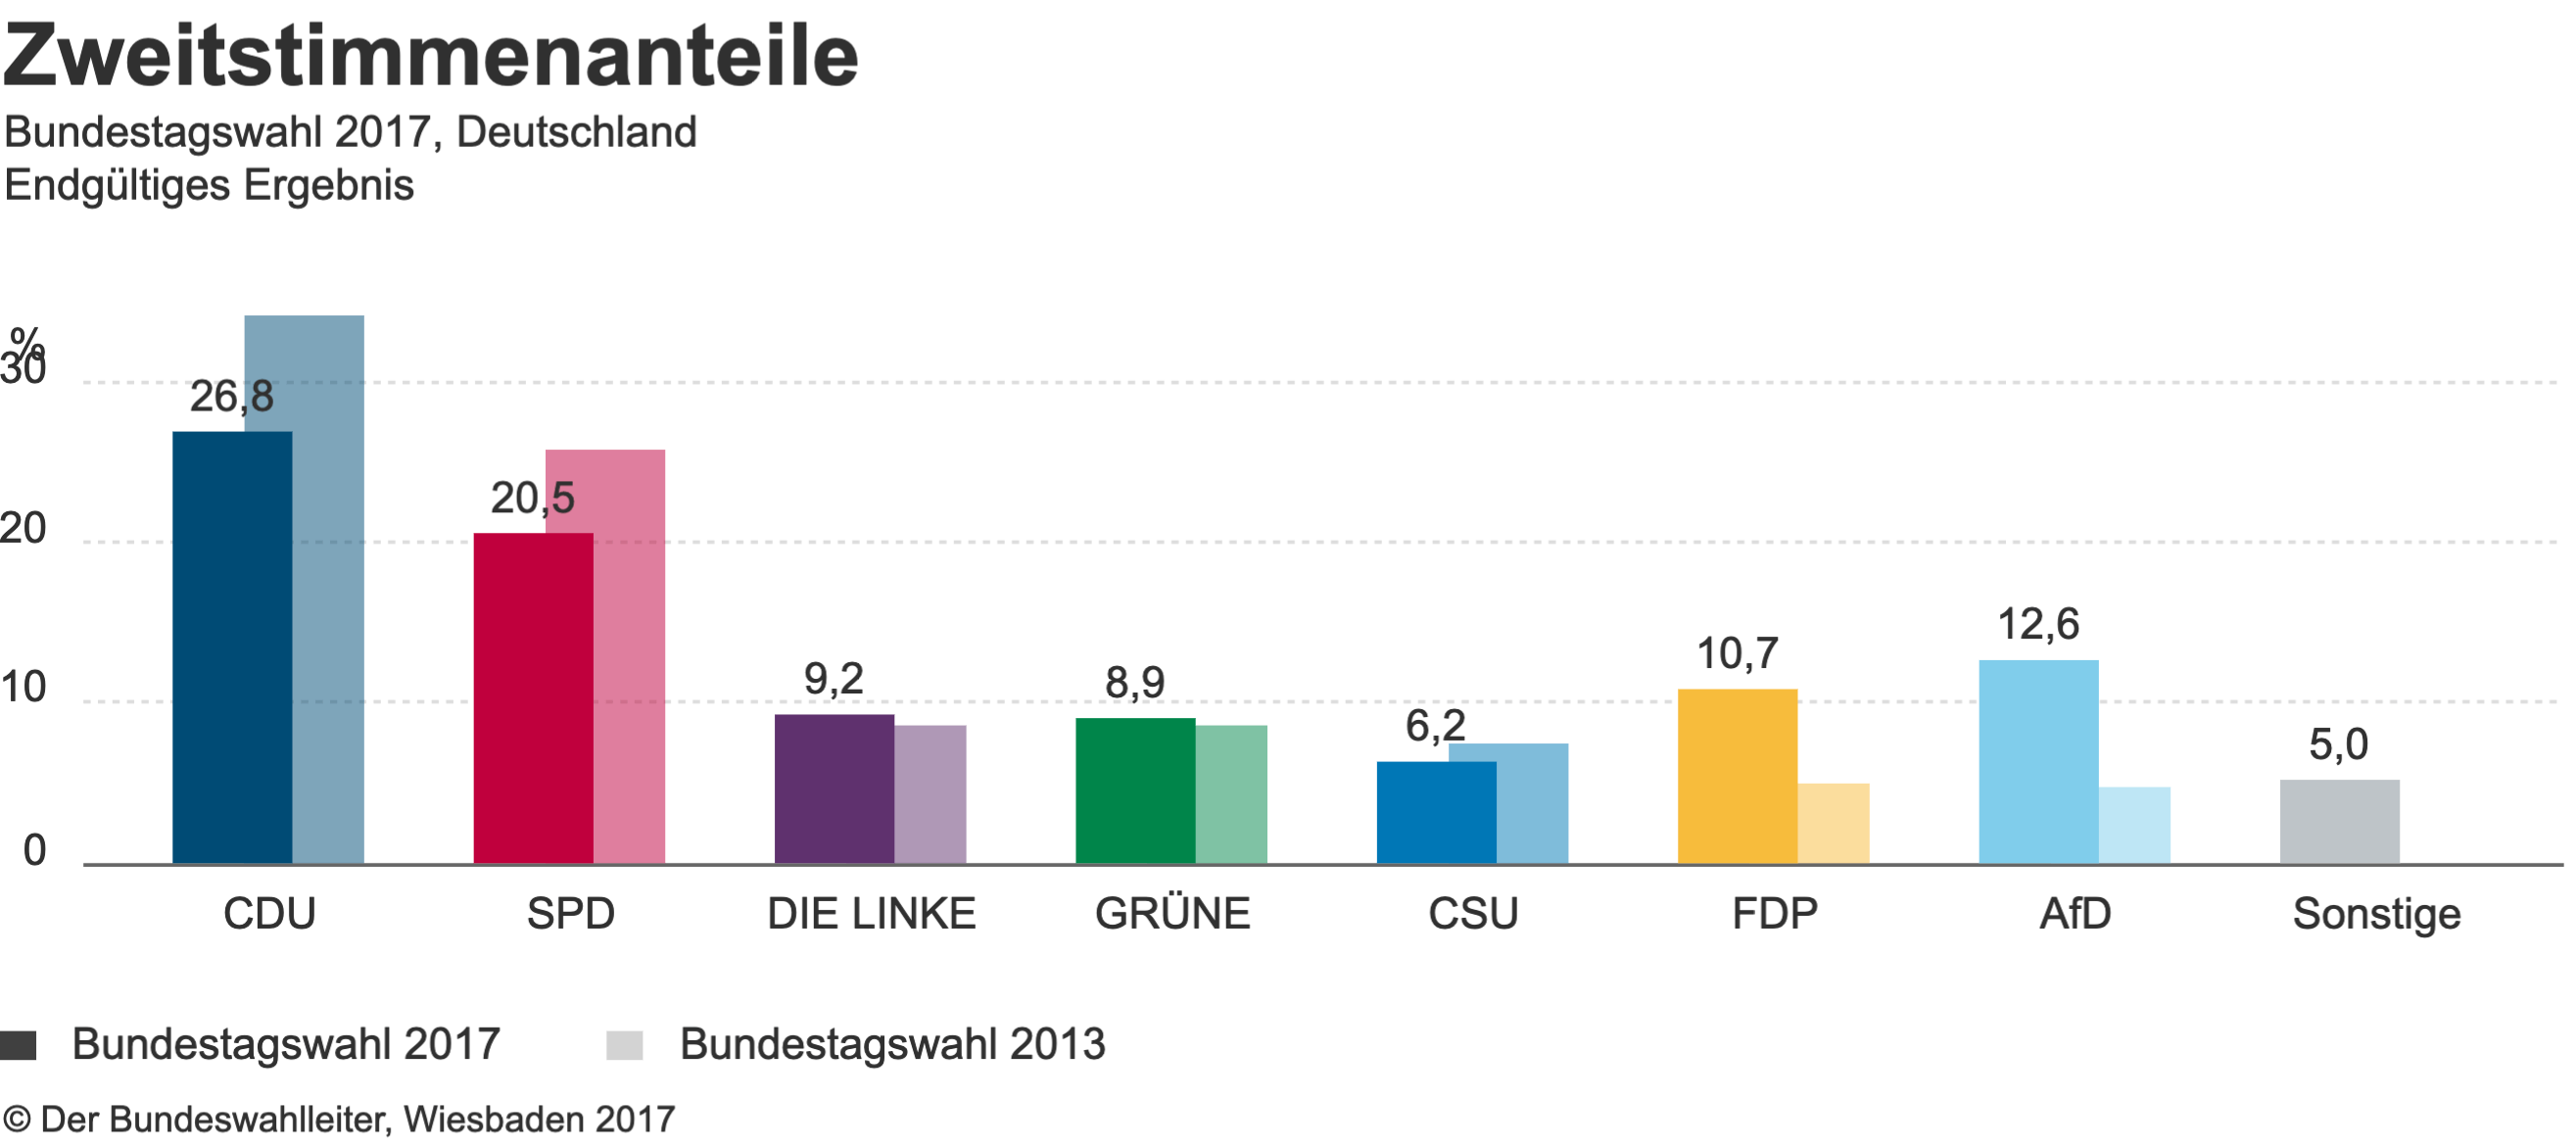
\includegraphics[width=0.9\textwidth]{data/images/ergebnisBtw17.png}
    \caption{Ergebnis der Bundestagswahl \num{2017} \autocite{noauthor_bundestagswahl_nodate}} \label{fig:ergebnisBtw17}
\end{figure}

Mit \SI{26.8}{\percent} konnte die \ac{CDU} mit starkem Verlust zur letzten Wahl die meisten Stimmen erlangen (zusammen als \ac{CDU}/\acs{CSU}-Fraktion \SI{32.9}{\percent}). Die \ac{SPD}, die ebenfalls im Vergleich zur Bundestagswahl \num{2013} an Stimmen verlor, kam auf \SI{20.5}{\percent}. Mit minimalen Steigerungen kamen die Linke auf \SI{9.2}{\percent} und die Grünen auf \SI{8.9}{\percent}. Sowohl die \ac{FDP} mit \SI{10.7}{\percent} als auch die \ac{AfD} mit \SI{12.6}{\percent} konnten ihre Ergebnisse deutlich steigern. Während es die \ac{AfD} durch dieses Ergebnis zum ersten Mal in den Bundestag schaffte, konnte die \ac{FDP} nach dem Ausscheiden \num{2013} erneut in den Bundestag einziehen. Die übrigen Parteien kamen kumuliert auf \SI{5}{\percent} der Stimmen.

\textcite{schmid_deutscher_2021} formuliert einige Erkenntnisse zu dem Ausgang der Wahl. So seien zum ersten Mal sieben Parteien und sechs Fraktionen im Bundestag vertreten. Dies könne als Zeichen für die weiter abnehmende Bindungskraft der Volksparteien \ac{CDU}, \ac{CSU} und \ac{SPD} gesehen werden. Zudem betont sie die starken Verluste von Union und \ac{SPD} mit starken Verlusten. Insbesondere habe die \ac{SPD} ihr schlechtestes Ergebnis seit \num{1949} erreicht.

Im Anschluss an die Wahl begonnen Sondierungsverhandlungen für eine mögliche \enquote{Jamaika-Koalition} zwischen Union, \ac{FDP} und Grünen. Nachdem diese seitens der \ac{FDP} abgebrochen wurden, bildete sich eine Große Koalition aus Union und \ac{SPD}. Damit gab es die längste Regierungsbildung in Deutschland aller Zeiten \parencite{schmid_deutscher_2021}.

\subsection{Heterogenität der Parteienlandschaft} \label{subsec:heterogenitätParteien}

Das Parteiensystem Deutschlands hat in den letzten Jahren einige Veränderungen durchlaufen. \textcite{niedermayer_entwicklung_2020} beschreibt allgemein eine Entwicklung von einem festen System mit zwei Partei (\ac{CDU} und \ac{SPD}) hin zu \enquote{einem pluralistischen System an der Grenze zum hochfragmentierten System}\parencite{niedermayer_entwicklung_2020}. Dabei sei besonders bei den Volksparteien ein schrittweiser Verlust der Zustimmung festzustellen. Hingegen finde eine Etablierung der Grünen als zweitstärkste Kraft statt. Zudem habe sich auch die \ac{AfD} fest verankert. Bei der \ac{FDP} und der Linken sei wenig Dynamik zu erkennen.

\textcite{engler_wettbewerb_2022} heben hervor, dass es zu vielen Themen eine große Bandbreite an alternativen Meinungen in der Opposition zur Regierung gebe. Beispielsweise stehen in der Klimapolitik Grüne und Linke für konsequentere Maßnahmen als die Regierung, während die \ac{AfD} entgegengesetzt positioniert sei. In der Debatte um \ac{COVID-19}-Maßnahmen ergebe sich ein ähnliches Bild, wobei sich auch die \ac{FDP} kritisch gegen einige Maßnahmen positioniert habe.

Nach \textcite{thomeczek_politische_2019} können die politischen Parteien in Deutschland grundlegend in zwei Lager eingeteilt werden: Ein \enquote{links-liberales} bestehend aus \ac{SPD}, Grünen und Linken, sowie ein \enquote{rechts-konservatives} oder \enquote{bürgerliches} aus \ac{CDU} und \ac{AfD}. Der \ac{FDP} wird als gesellschaftspolitisch liberale, aber wirtschaftspolitisch rechte Partei eine Sonderrolle zugeschrieben. Zudem beobachten \textcite{thomeczek_politische_2019}, dass es zwischen den Parteien Unterschiede gebe, inwieweit sie intern kohärent sind. Die Volksparteien \ac{SPD} und \ac{CDU} weisen dabei durchschnittlich weniger hohe Agreement-Index-Werte -- ein Maßstab, wie stark die Positionen der Mitglieder übereinstimmen -- auf als die anderen Parteien.

Die Verteilung der Positionen innerhalb einer Partei betrachtet auch \textcite{saltzer_bundestagswahl_2022}. \autoref{fig:positionierungAusgewaehlterKanidaten} zeigt die Verortung von Kandidaten für die Bundestagswahl 2021 nach Partei. Die x-Achse stellt dabei die Position in der politischen Links-Rechts-Skala und die y-Achse die Zustimmung zu Regierung beziehungsweise Opposition.

\begin{figure}[H]
    \centering
    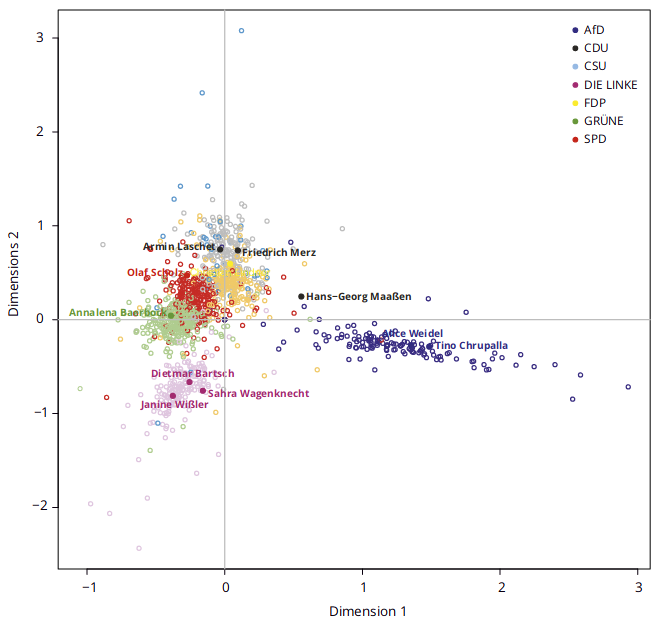
\includegraphics[width=0.5\textwidth]{data/images/positionierung_ausgewaehlter_kandidaten.png}
    \caption[Positionierung ausgewählter Kandidaten \autocite{saltzer_bundestagswahl_2022}]{Positionierung ausgewählter Kandidaten innerhalb eines zweidimensionalen politischen Raums \autocite{saltzer_bundestagswahl_2022}} \label{fig:positionierungAusgewaehlterKanidaten}
\end{figure}

Es fällt auf, dass Linke und vor allem \ac{AfD} klar abgetrennt sind von der Positionierung der anderen Parteien. \ac{CDU}, \ac{CSU}, \ac{FDP}, \ac{SPD} und Grüne liegen um den Ursprung des Koordinatensystems herum eng beieinander und überschneiden sich dabei auch.

Kandidaten der Union und \ac{FDP} liegen im Schnitt in der Mitte der Links-Rechts-Skala. Dabei liegt die Regierungs-Zustimmung der Union höher. Im Vergleich zur \ac{FDP} ist die \ac{SPD} weiter links positioniert. Die Kandidaten der Grünen sind noch weiter links eingezeichnet und neutral auf der y-Achse. Die Linken befinden sich ähnlich weit links wie die Grünen, sind aber deutlich eher der Opposition zugeneigt. Die \ac{AfD} ist die einzige Partei, die nach der gegebenen Darstellung rechts der Mitte aufzufinden ist und dabei eher der Opposition nahesteht.

Auffällig ist, dass der Bereich, in dem \ac{AfD}-Kandidaten auf der Links-Rechts-Skala eingeordnet werden, deutlich größer ist als bei den anderen Parteien. Dies legt eine niedrige interne Einigkeit nahe.

\subsection{Besondere Ereignisse im Untersuchungszeitraum} \label{subsec:besondereEreignisse}

\textcite{schmid_deutscher_2021} stellt wichtige öffentlichkeitswirksame Ereignisse während der 19. Wahlperiode des deutschen Bundestages dar. Darunter fällt zunächst die \ac{COVID-19}-Pandemie, der Auswirkungen und der Umgang mit diesen nach den ersten Ansteckungsfällen Anfang 2020 zu einem zentralen Thema in Politik und Gesellschaft wurden. Im Juli 2021 kam es in Teilen von Nordrhein-Westfalen und Rheinland-Pfalz zu einer schweren Flutkatastrophe. Kurz vor Ende der Legislaturperiode wurde zudem der Einsatz der Bundeswehr in Afghanistan beendet, nachdem eine Machtübernahme der Taliban erfolgt war.

Neben der Bundestagswahl 2017 fand als weitere bundesweite Wahl die Wahl zum Europäischen Parlament am 29. Mai 2019 statt. Zudem wurden 13 Landtagswahlen ausgerichtet.

\subsection{Themenschwerpunkte} \label{subsec:themenschwerpunkte}

\textcite{engler_wettbewerb_2022} untersuchen die Themenschwerpunkte in politischen Debatten während der 19. Wahlperiode. Der Verlauf der Relevanz ausgewählter Themen basierend auf Umfragen der Forschungsgruppe Wahlen ist in \autoref{fig:themenkonjunktur} abgebildet.

\begin{figure}[H]
    \centering
    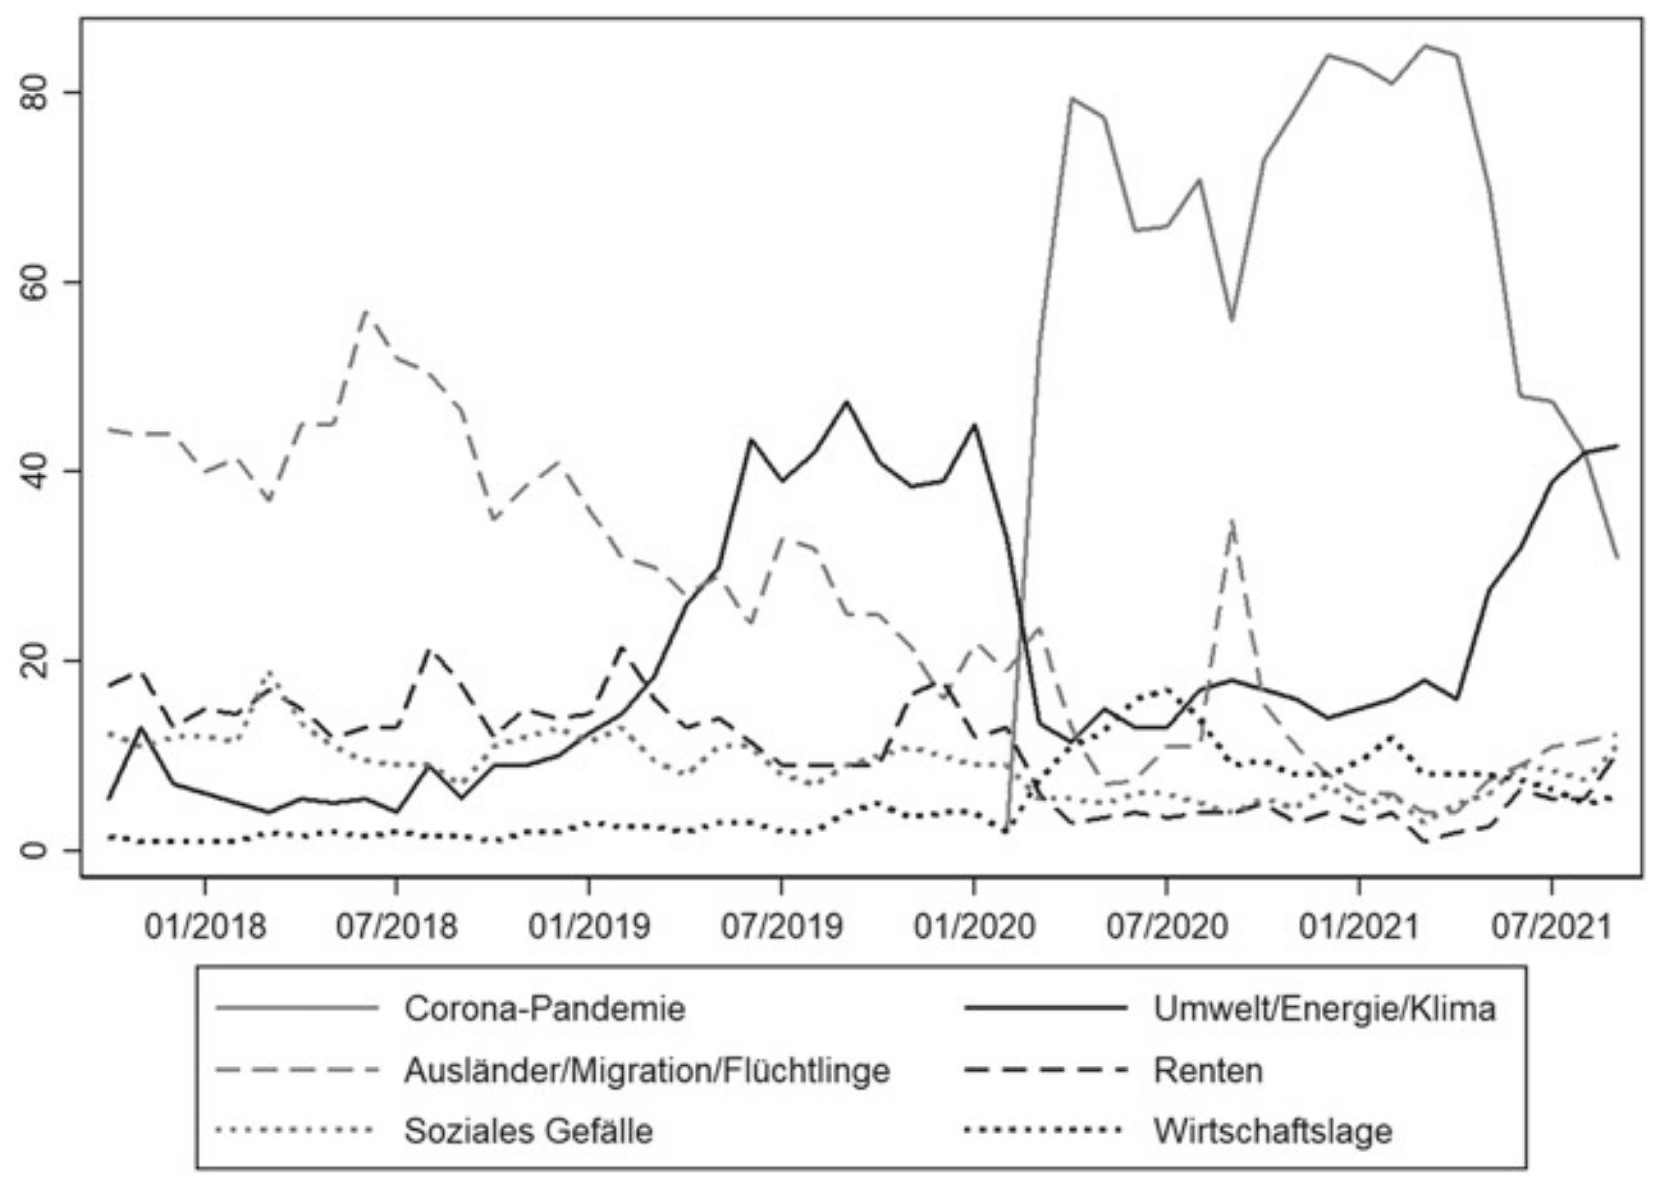
\includegraphics[width=0.8\textwidth]{data/images/themenkonjunktur.png}
    \caption{Verlauf der wichtigsten politischen Themen während der 19. Wahlperiode \autocite{engler_wettbewerb_2022, forschungsgruppe_wahlen_forschungsgruppe_nodate}} \label{fig:themenkonjunktur}
\end{figure}

Zu Beginn der Legislaturperiode war das Thema der Migrationspolitik am wichtigsten. Die Relevanz ist hat jedoch stetig abgenommen, bis das Thema ab 2020 eher untergeordnet war. Der Themenbereich Umwelt, Energie und Klima wurde ab 2019 immer wichtiger und war zeitweise das Thema mit der meisten Relevanz. Nach der Flutkatastrophe 2021 wurde diesem Bereich wieder vermehrt Bedeutung zugesprochen. Nach dem Ausbruch der Pandemie war diese schlagartig mit Abstand am wichtigsten, bis sich die Lage 2021 wieder beruhigte. Während des gesamten Zeitraums rückten wirtschafts- und sozialpolitische Themen in den Hintergrund.

Nach \textcite{niedermayer_entwicklung_2020} waren im Betrachtungszeitraum vor allem die Flüchtlingskrise sowie das Thema Klimawandel und Energiewende von Bedeutung. Die Relevanz des zweiten Themas können man am Dieselskandal, der Hitzewelle im Sommer \num{2018} sowie der Popularität der Protestbewegung \enquote{Fridays for Future} erkennen.

\section{Repräsentationsformen von Text}

% TODO: Either describe specific models or the underlying architecture (e.g. fasttext or n-gram method)

Um \ac{ML} und andere Analysen auf Text anzuwenden, ist es notwendig diesen in maschinenlesbare Sprache umzuwandeln. Abhängig von der Methodik wird die Integrität der syntaktischen und semantischen Beziehungen beeinflusst \autocite{kowsari_text_2019, jurafsky_speech_2023}.

Herkömmliche Methoden wie \ac{BoW} und \ac{TF-IDF} generieren unkomprimierte Vektoren und skalieren linear mit der Anzahl an einzigartigen Wörtern. Diese Verfahren können jedoch nicht den Kontext innerhalb eines Satzes analysieren. Ein alternativer Ansatz ist die Repräsentation mittels kontextabhängigen Verfahren. Mittels neuronalen Netzen können Zusammenhänge innerhalb eines Satzes erkannt werden. Beispielhafte Implementierungen sind \ac{LSTM}-Netzwerke, als auch \ac{ELMo}.

% TODO: Transformer Modelle

Worteinbettungen (engl. Word Embeddings) repräsentieren eine zentrale Rolle, bei der Analyse und dem Training von \ac{NLP} Modellen. Diese bilden einzigartige Wörter mittels mehrdimensionalen Vektoren\footnote{Häufig bestehen Word Embeddings aus \num{300} Dimensionen} ab. Abhängig vom Verfahren sind die resultierenden Vektoren komprimiert oder unkomprimiert. Worteinbettungen ermöglichen es, Wörter mit einer ähnlichen Semantik und Syntax im mehrdimensionalen Raum nah beieinander zu gruppieren.

Die unterschiedlichen Verfahren können meist auf Wort-, Satz- oder Dokumentebene angewendet werden.

\subsection{Kontextunabhängig}

\ac{BoW} und \ac{TF-IDF} extrahieren Informationen über die Häufigkeit einzelner Wörter. Beide Verfahren geben somit Aufschluss über den Inhalt und Themen einzelner Texte. Jedoch ermöglichen die Verfahren nicht, den genauen Kontext, Grammatik und Satzbau zu analysieren. 

% TODO: Beide Verfahren zu einer großen Anzahl an Features (unkompromiert)

\subsubsection*{N-Gram}

N-Grams sind die Grundlage für Verfahren wie \ac{BoW} und Fasttext. Bei dieser Methode werden Zeichen (Wortebene) oder Wörter (Satzebene) in Tupel mit der Länge \texttt{n} unterteilt \autocite[5]{kowsari_text_2019}. Die Reihenfolge der Wörter bleibt dabei unverändert. 

Nach \textcite[5]{kowsari_text_2019} sind häufig verwendete Werte \num{2} und \num{3}.

\subsubsection*{\acl{BoW}} 

\ac{BoW} ist eine der simpleren Repräsentationsformen, da es lediglich die Häufigkeit von einzigartigen Wörtern berechnet \autocite[6]{kowsari_text_2019}. Im ersten Schritt des Verfahrens, wird ein Satz oder Dokument in eine Menge an 1-Grams transformiert. Anschließend wird die Liste auf die einzigartigen Wörter reduziert. Schlussendlich wird gezählt, wie häufig die einzigartigen Wörter (engl. Features) auftreten. Die daraus entstehende Tabelle wird auch \ac{BoF} genannt.

% TODO: Beispiel
% TODO: Limitation -> Das ist gut & Ist das Gut

\subsubsection*{\acl{TF-IDF}}

Neben der reinen Häufigkeit berücksichtigt \ac{TF-IDF} außerdem die Häufigkeit eines Wortes für eine Sammlung an Dokumenten \autocite[7]{kowsari_text_2019}. Damit ist es möglich Wörter, aus Wortgruppen wie Artikeln, Präpositionen, Konjunktionen von relevanten Wörtern (meist Adjektive, Verben und Nomen) zu trennen.

\[\mathrm{tfidf}(t,d,D) = \frac{f_{t,d}}{{\sum_{t' \in d}{f_{t',d}}}} \cdot \log \frac{N}{|\{d \in D: t \in d\}|}\]

Dafür wird zunächst die relative oder absolute Häufigkeit eines Wortes innerhalb eines Dokumentes berechnet. Außerdem wird die Häufigkeit in anderen Dokumenten berechnet. Der sich daraus ergebene Wert gibt Auskunft darüber, ob es sich um ein generell häufiges Wort oder nicht handelt.

\subsubsection*{Word2Vec, FastText, GloVe (CBOW)}

% TODO: Beispiel -> König - Mann + Frau = Königin
% TODO: Problem -> Bank liefert Vektor zwischen Parkbank und Geldinstitut
% TODO: Möglicher Bias -> Arzt - Mann + Frau = Krankenschwester
% TODO: Nur nahestehende Stymbolde werden als Kontext interpretiert

CBOW:

\begin{figure}[H]
    \centering
    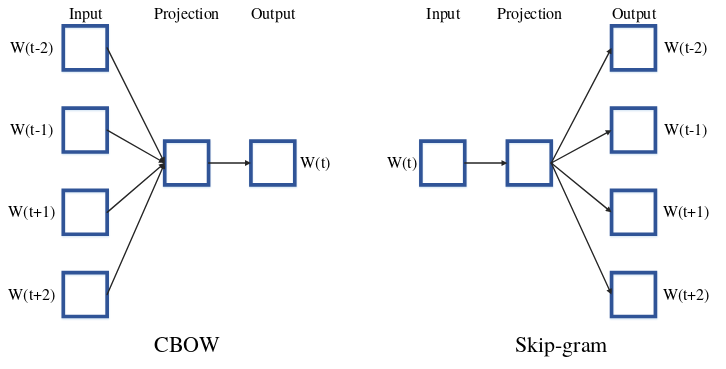
\includegraphics[width=0.6\textwidth]{data/images/materials_and_methods/cbow_skip_gram.png}
    \caption{\autocite[8]{kowsari_text_2019}}
    \label{fig:cbow_skip_gram}
\end{figure}

Fasttext:

Anders als andere herkömmliche Worteinbettungen nutzt Fasttext keine gesamten Wörter, sondern Zeichen-basierte n-grams (meist tri-grams) \autocite[9]{kowsari_text_2019}.

Lorem Ipsum

\subsection{Kontextabhänig}

Um syntaktische und semantische Beziehungen zu erkennen, ist es notwendig, nicht nur den Satzbau, sondern auch die Bedeutung einzelner Wörter schon mittels der Methodik zur Transformation zu berücksichtigen. Kontextabhängige Worteinbettungen verwenden meist einen Speicher an vorherigen Wörtern, um den Kontext zu darauffolgenden Wörtern herzustellen.

\subsubsection*{LSTM}

Lorem Ipsum

\subsubsection*{ELMo}

Lorem Ipsum

\subsection{Transformer}

% TODO: Add and describe models used for modeling

\subsubsection*{BERT}

Lorem Ipsum

\section{Feature Engineering}

\subsection*{Analyse der Stimmung}

% TODO: Explain sentiment model and accuracy

Die Arbeit von \textcite{guhr_training_2020} zeigt, wie sich Texte anhand ihrer Stimmung -- Positiv, Neutral, oder Negativ -- mittels \ac{BERT} klassifizieren lassen. Für das Training nutzten die Autoren acht unterschiedliche Datensätze, die insgesamt \num{5.3} Millionen Einträge umfassen. Neben dem \ac{BERT}-Modell wurde ebenfalls ein Modell mittels FastText tainiert, dieses Performte jedoch leicht schlech

Mittels eines Modells, das auf der Basis von \ac{BERT} trainiert wurde, lässt sich die Stimmung in verschiedenen Texten ermitteln \autocite{guhr_training_2020}. Das Modell ist auf der Basis von PotTS (Sidarenka, 2016), SB10k (Cieliebak et al., 2017), GermEval-2017 (Wojatzki et al., 2017), holidaycheck.de, filmstarts.de, Scare (Sänger et al., 2016) und Leipzig corpora collection (Goldhahn et al., 2012) trainiert worden. Insgesamt umfassen der verwendete Datensatz \num{5.3} Millionen Einträge, die mit \textit{positiv}, \textit{neutral} oder \textit{negativ} gekennzeichnet sind \autocite[1629]{guhr_training_2020}.

\section{Zusammenfassung}
